\documentclass{article}

% CIS model using deformations of an elastic chebyshev net.

\usepackage[utf8]{inputenc}

% Math symbols
\usepackage{amsmath}
\usepackage{amssymb}
\usepackage{siunitx} % Format numbers in scientific notation.
\sisetup{output-exponent-marker=\ensuremath{\mathrm{e}}} % This forces latex to use the "calculator" version of scientific notation with `E` rather than a true typset exponent.

% Tables.
\usepackage{multirow}
\usepackage{booktabs}

% Figures.
\usepackage{graphicx}
\graphicspath{{figures/}}
\usepackage{caption}
\usepackage{subcaption}

% Citation/Bibliograph.
\usepackage{natbib} % Include `\cite` command.

%% BEGIN PAPER

\title{AM254 Final Project Proposal}
\author{Noah Toyonaga}

\begin{document}

\maketitle
\tableofcontents

\section{Problem Statement}

This project concerns the dynamics of (1D) arrays of masses densely interconnected by springs. 

As a familiar entry point, we can consider the dynamics of a 1D chain of masses and springs (we might call this a ``sparse'' array), of the type typically encountered in an introductory physics curriculum. 
See  fig. \ref{fig:1D_chain}.
Letting  $u$ represent the displacement of the mass $i$ rom its equilibrium, 
the equations of motion for this system can be concisely written in the form \ref{eq:sparse_eom}. 
The normal modes of this system are well understood, and correspond to the modes of a discretized wave equation (given appropriate boundary conditions).

\begin{equation}
	\label{eq:sparse_eom}
	m u_{tt} = \underbrace{
		\begin{pmatrix}
			-2k & k & 0 &\cdots & 0 \\
			k & -2k & k & \cdots & 0 \\
			0 & k & -2k & \cdots & \vdots \\
			\vdots &&& \ddots & k \\
			0 & \cdots & & k & -2k \\
		\end{pmatrix}
	}_{\textbf{A}}u
\end{equation}


Now, we consider an array that has non-nearest neighbor connections (randomly distributed), as in \ref{fig:1D_dense}.
The equations of motion of this system can again be written in the form of a matrix equation \ref{eq:dense_eom},
where the matrix $\star{A}$ no longer takes the form of a block diagonal as $A$.
It will in general be dense, reflecting the connection pattern.

\begin{equation}
	\label{eq:dense_eom}
	m u_{tt}  = \star{A}u
\end{equation}

The goal of this project is to characterize the dynamics of this system, primarily by studying the 
leading eigenmodes of the dense model (\ref{eq:dense_eom}) using the techniques presented in class (spectral/TAP).
In particular, I am interested in studying the appearance of mode localization under different types of connection ``noise''.
It will be of interest to study both the modes of the puresly dense system, 
as well as the sparse system with dense connections added as a type of noise 
(with the strength of this noise corresponding to the physcial stiffness $k$ of non-nearest-neighbor bonds).

If I have sufficient time I would also like to think about perturbations to the system in the form of ``breaking bonds'', 
i.e. setting the spring constant of various bonds to 0. 
This paves the way towards an understanding of the dynamics of damaged networks in physical systems. 

\begin{figure}
\begin{center}
	\begin{subfigure}[]{.45\textwidth}
	\begin{center}
		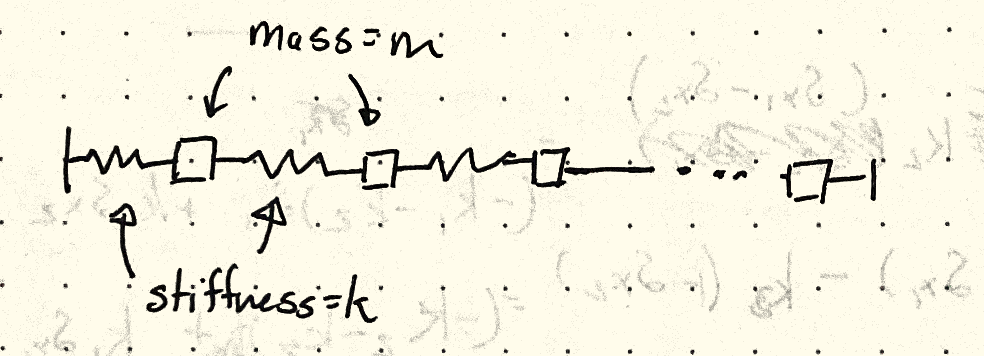
\includegraphics[width=\textwidth]{1D_sparse.png}
	\end{center}
	\caption{sparse}
	\label{fig:1D_chain}
	\end{subfigure}
	\hfill
	\begin{subfigure}[]{.45\textwidth}
	\begin{center}
		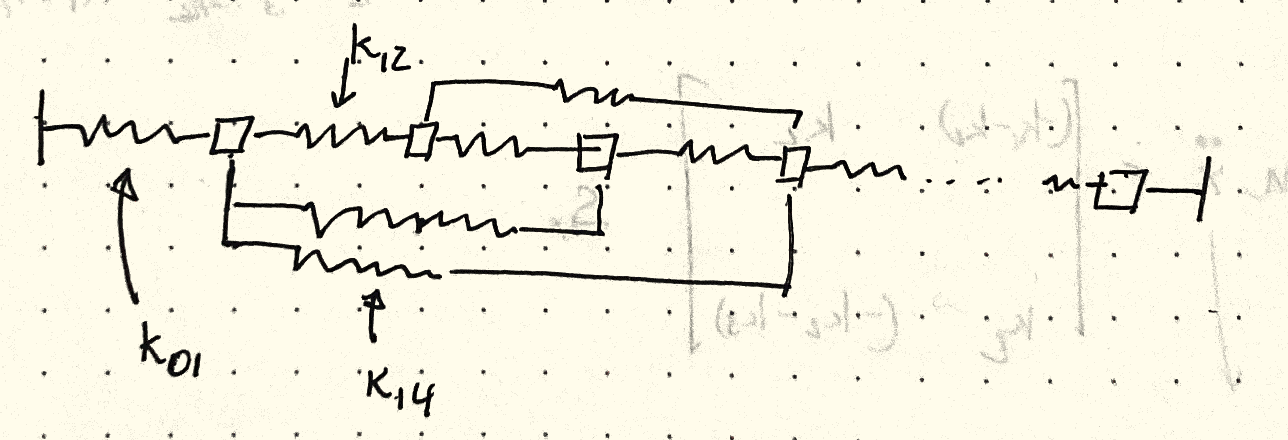
\includegraphics[width=\textwidth]{1D_dense.png}
	\end{center}
	\caption{dense}
	\label{fig:1D_dense}
	\end{subfigure}
\end{center}
\caption{Representations of a sparse and dense 1D array of springs and masses. In general the springs may have different stiffnesses $k_{ij}$.}
\label{fig:spring_arrays}
\end{figure}


\section{Motivation and Broader Context}
I believe this project can be motivated by (at least) two different contexts.


\subsection{Soft matter and Network Materials}

Separately, models of ``dense'' interconnection may be applicable to soft matter systems contituted by networks.
Examples of such network materials include microbiological aggregates (actin filaments with myosin crosslinks, collagen) as well as engineered materials (hydrogels, elastomers).
Of course, in these situatiosn and others, the networks are 2D and so geometry plays a central role in determining the distribution of forces and concommitant dynamics (as opposed to the purely topological setting of 1D). 

\subsection{Noisy Laplacian}

As noted in the previous section, the chain of masses connected by springs
naturally appears as the discretization of the wave equation 
(or, equivalently, the continuum model for an infinite mass-spring system is the wave equation).


In this context, we can think of the addition of non-nearest-neighbor springs as modifications to the continuum laplacian operator as in \ref{eq:noisy_laplacian}.

\begin{equation}\label{eq:noisy_laplacian}
	\frac{\partial^3}{\partial x^2} \equiv \nabla^2 \rightarrow \nabla^2 + \vec{v}
\end{equation}


\end{document}


